In this chapter, we turn to the problem of reasoning over structured contexts, 
towards comprehending compositional language. We take a semantic parsing 
approach for Question Answering on (semi) structured
domains, and describe an encoder-decoder framework, where we set explicit type 
constraints on the decoder. Following the overarching theme of this thesis, we 
seek to build end-to-end models for these QA problems
as well. Accordingly, we assume that the only direction supervision we get is 
from the answers at the end (i.e., our semantic parser is weakly supervised).

\section{Type Constrained Neural Semantic Parser}
\begin{figure}
\centering
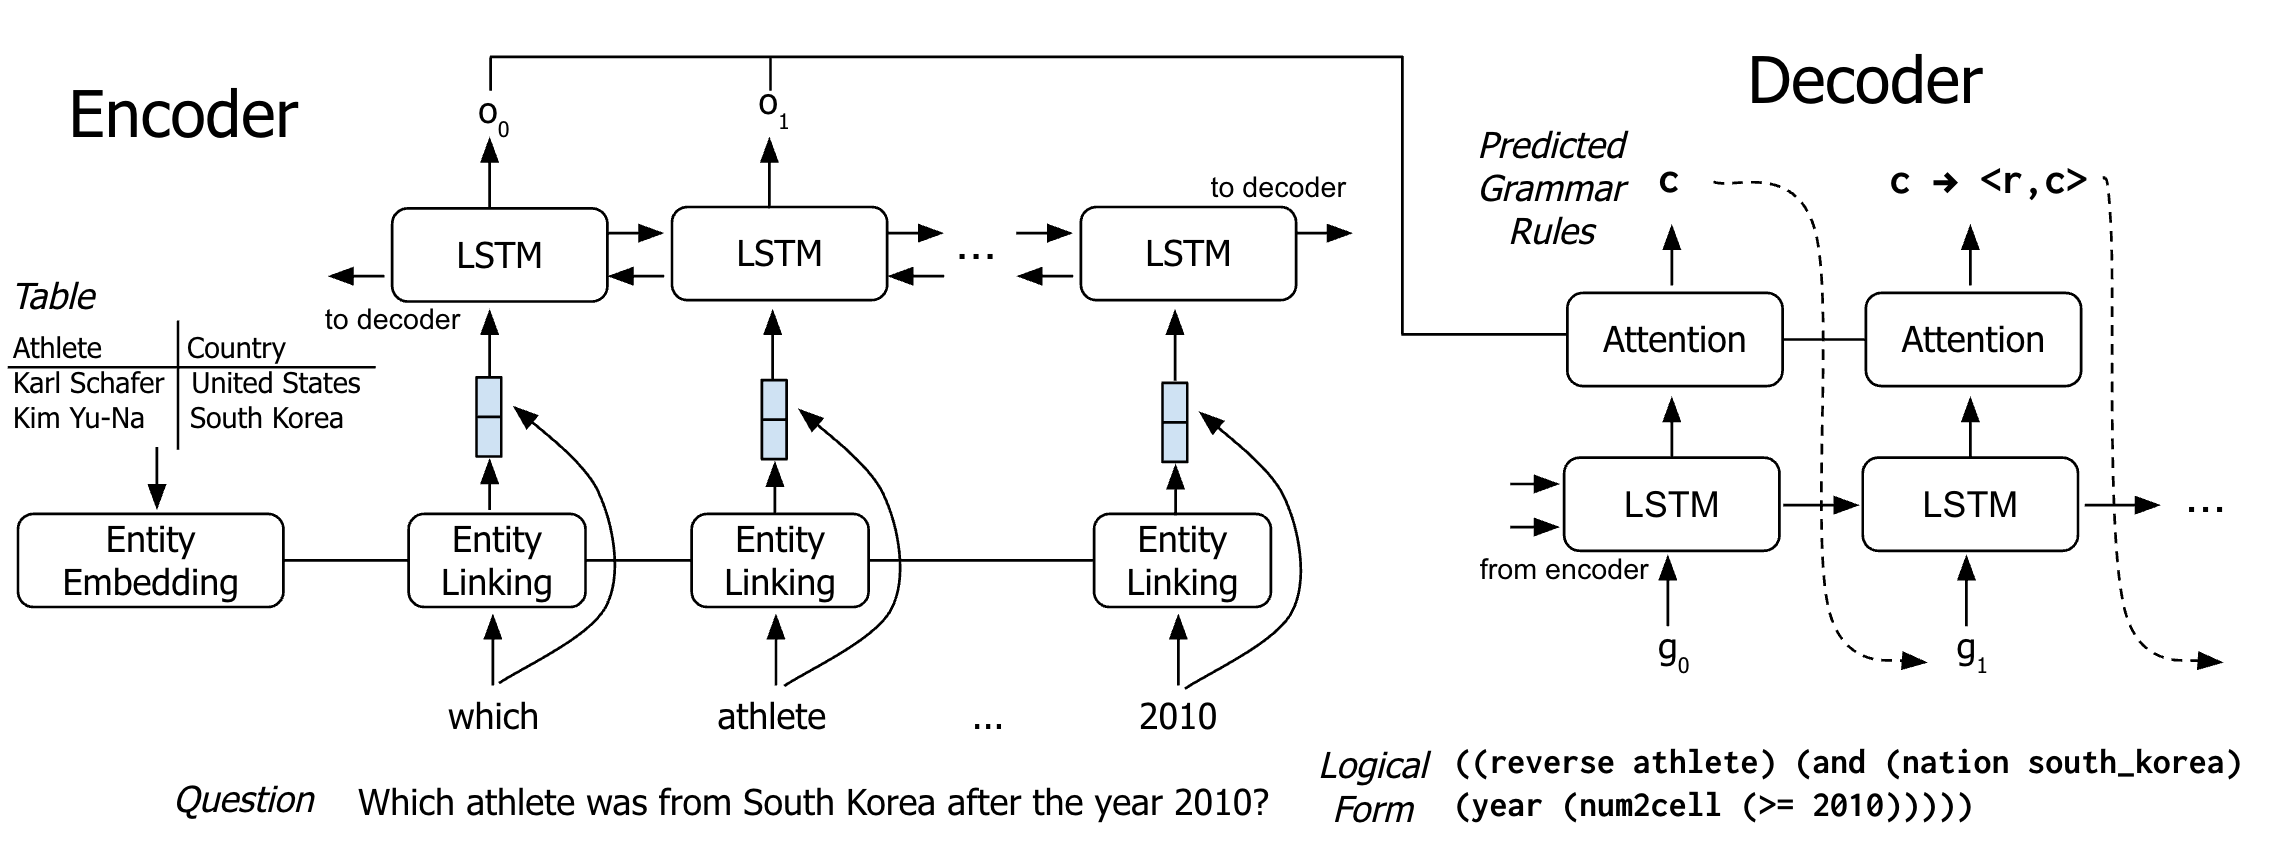
\includegraphics[width=6in]{figures/type_constrained_nnsp.png}
\caption{Overview of our type-constrained neural semantic parsing model}
\label{fig:nnsp_model}
\end{figure}

This section describes our semantic parsing model.
The input to our model is a natural language question and a context in which it 
is to be answered.
The model predicts the answer to the question by semantically parsing it to a 
logical form then executing it against the context.

Our model follows an encoder-decoder architecture, using recurrent neural 
networks with Long Short Term Memory (LSTM) cells~\citep{hochreiter1997long}. 
The input question and table entities are first encoded as vectors that are 
then decoded into a logical form (Figure \ref{fig:nnsp_model}).
We make two significant additions to the standard encoder-decoder architecture.
First, the encoder includes a special entity embedding and linking module that 
produces a \emph{link embedding} for each question token that represents the 
table entities it links to (Section \ref{sec:nnsp_encoder}).
These link embeddings are concatenated with word embeddings for each question 
token, then encoded with a bidirectional LSTM.
Second, the action space of the decoder is defined by a \emph{type-constrained 
grammar} which guarantees that generated logical forms satisfy type constraints 
(Section \ref{sec:nnsp_decoder}).
The decoder architecture is simply an LSTM with attention that predicts a 
sequence of generation actions within this grammar.

We train the parser using question-answer pairs as supervision, using an 
objective based on enumerating logical forms via dynamic programming on 
denotations \citep{pasupat2016inferring} (Section \ref{sec:nnsp_training}). This 
objective function makes it possible to train neural models with 
question-answer supervision, which is otherwise difficult for efficiency and 
gradient variance reasons.

\subsection{Encoder}
\label{sec:nnsp_encoder}

The encoder network is a standard bidirectional LSTM augmented with an entity 
embedding and linking module.

\paragraph{Notation.}
Throughout this section, we denote entities as $e$, and their corresponding 
types as $\tau(e)$. The $i^{\text{th}}$ token in a question is denoted $q_i$. 
We use $v_w$ to denote a learned vector representation (embedding) of word $w$, 
e.g., $v_{q_i}$ denotes the vector representation of the $i$th question token. 
Finally, we denote the set of all entities as $E$, and all entities belonging 
to a type $\tau$ as $E_{\tau}$. The entities $E$ include all of the entities 
from the table, as well as numeric entities detected in the question by NER. 

\paragraph{Entity Embedding.}
The encoder first constructs an embedding for each entity in the knowledge 
graph given its type and position in the graph. 
Let $W(e)$ denote the set of words in the name of entity $e$ and $N(e)$ the 
neighbors of entity $e$ in the knowledge graph.
Each entity's embedding $r_e$ is a nonlinear projection of a type vector 
$v_{\tau(e)}$ and a neighbor vector $v_{N(e)}$:
\begin{align}
    v_{N(e)} &= \sum_{e' \in N(e)}\sum_{w \in W(e')}v_w \\
    r_e &= \tanh\big(P_\tau v_{\tau(e)} + P_N v_{N(e)}\big)
\end{align}
The type vector $v_{\tau(e)}$ is a one-hot vector for $\tau(e)$, with dimension 
equal to the number of entity types in the grammar. The neighbor vector 
$v_{N(e)}$ is simply an average of the word vectors in the names of $e$'s 
neighbors. $P_\tau$ and $P_N$ are learned parameter matrices for combining 
these two vectors.

\paragraph{Entity Linking.}
This module generates a \emph{link embedding} $l_{i}$ for each question token 
representing the entities it links to.
The first part of this module generates an entity linking score $s(e,i)$ 
for each entity $e$ and token index $i$:

\begin{align}
s(e,i) & = \max_{w \in W(e)} v_w^\intercal v_{q_i} + \psi^\intercal \phi(e,i)
\end{align}

This score has two terms. The first represents similarity in word embedding 
space between the token and entity name, computed as function of the embeddings 
of words in $W(e)$ and the word embedding of the $i$th token, $v_{q_i}$. The 
second represents a linear classifier with parameters $\psi$ on features 
$\phi(e,i)$.
The feature function $\phi$ contains only a few features: exact token match, 
lemma match, edit distance, an NER indicator feature, and a bias feature.
It also includes token and lemma features coming from the neighbors of the node
that originally matches the token. We found that features were an effective way
to address sparsity in the entity name tokens, many of which appear too 
infrequently
to learn embeddings for.

Finally, the entity embeddings and linking scores are combined to produce a 
link embedding for each token.
The scores $s(e,i)$ are then fed into a softmax layer over all entities $e$ of 
the same type, and the link embedding $l_{i}$ is an average of entity vectors 
$r_e$ weighted by the resulting distribution.
We include a null entity, $\varnothing$, in each softmax layer to permit the 
model to identify tokens that do not refer to an entity. The null entity's 
embedding is the all-zero vector and its score $s(\varnothing, \cdot) = 0$.

\begin{align}
%p(e | q_i, \tau(e)) & = \frac{\exp{s(e,q_i)}}{1 + \sum_{e} \exp{s(e,q_i)}} \\
%v_i & = \sum_{\tau} \sum_e v_e p(e | q_i, \tau)
p(e | i, \tau) & = \frac{\exp{s(e,i)}}{\sum_{e'\in E_\tau \cup \{\varnothing\}} 
\exp{s(e',i)}} \\
l_{i} & = \sum_\tau \sum_{e \in E_\tau} r_e p(e | i, \tau)
\end{align}

\paragraph{Bidirectional LSTM.}
We concatenate the link embedding $l_i$ and the word embedding $v_{q_i}$ of 
each token in the question, and feed them into a bidirectional LSTM:

\begin{align}
x_i &= \begin{bmatrix} l_{i} \\ v_{q_i} \end{bmatrix} \\
(o^f_i, f_i) &= \text{LSTM}(f_{i-1}, x_i) \\
(o^b_i, b_i) &= \text{LSTM}(b_{i+1}, x_i) \\
o_i &= \begin{bmatrix} o^f_i \\  o^b_i \end{bmatrix}
\end{align}

This process produces an encoded vector representation of each token $o_i$. The 
final LSTM hidden states $f_n$ and $b_{-1}$ are concatenated  and used to 
initialize the decoder.

\subsection{Decoder}
\label{sec:nnsp_decoder}

The decoder is an LSTM with attention that selects parsing actions from a 
grammar over well-typed logical forms.

\paragraph{Type-Constrained Grammar.} The parser maintains a state at each step 
of decoding that consists of a logical form with typed \emph{holes}.
A hole is a tuple \hole{\tau}{\Gamma} of a type $\tau$ and a \emph{scope} 
$\Gamma$ that contains typed variable bindings, $(x:\alpha) \in \Gamma$.
The scope is used to store and generate the arguments of lambda expressions. 
The grammar consists of a collection of four kinds of production rules on holes:

\begin{enumerate}
    \item \textbf{Application} 
\hole{\tau}{\Gamma}$\rightarrow$\pred{(}\hole{\func{\beta}{\tau}}{\Gamma}~\hole{
\beta}{\Gamma}\pred{)} rewrites a hole of type \type{\tau} by applying a 
function from \type{\beta} to \type{\tau} to an argument of type \type{\beta}. 
We also permit applications with more than one argument.
    \item \textbf{Constant} \hole{\tau}{\Gamma}$\rightarrow$\pred{const} where 
constant \pred{const} has type \type{\tau}. This rule generates both 
context-independent operations such as \pred{argmax} and context-specific 
entities such as \pred{united\_states}.
    \item \textbf{Lambda} \hole{\func{\alpha}{\tau}}{\Gamma}$\rightarrow 
\lambda x.$ \hole{\tau}{\Gamma \cup \{(x : \alpha)\}} generates a lambda 
expression where the argument has type \type{\alpha}. $x$ is a fresh variable 
name.
    \item \textbf{Variable} \hole{\tau}{\Gamma}$\rightarrow x$ where $(x : 
\tau) \in \Gamma$. This rule generates a variable bound in a 
previously-generated lambda expression that is currently in scope.
\end{enumerate}

We instantiate each of the four rules above by replacing the type variables 
$\tau, \alpha,\beta$ with concrete types, producing, e.g., $\hole{c}{\Gamma} 
\rightarrow (\hole{\func{r}{c}}{\Gamma}~\hole{r}{\Gamma})$ from the application 
rule.
The set of instantiated rules is automatically derived from a corpus of logical 
forms, which we in turn produce by running dynamic programming on denotations 
(see Section \ref{sec:nnsp_training}).
Every logical form can be derived in exactly one way using the four kinds of 
rules above; this derivation is combined with the (automatically-assigned) type 
of each of the logical form's subexpressions to instantiate the type variables 
in each rule.
We then filter out constant rules that generate context-specific entities 
(which are 
handled specially by the decoder) to produce a 
context-independent grammar.

\begin{figure}
\centering
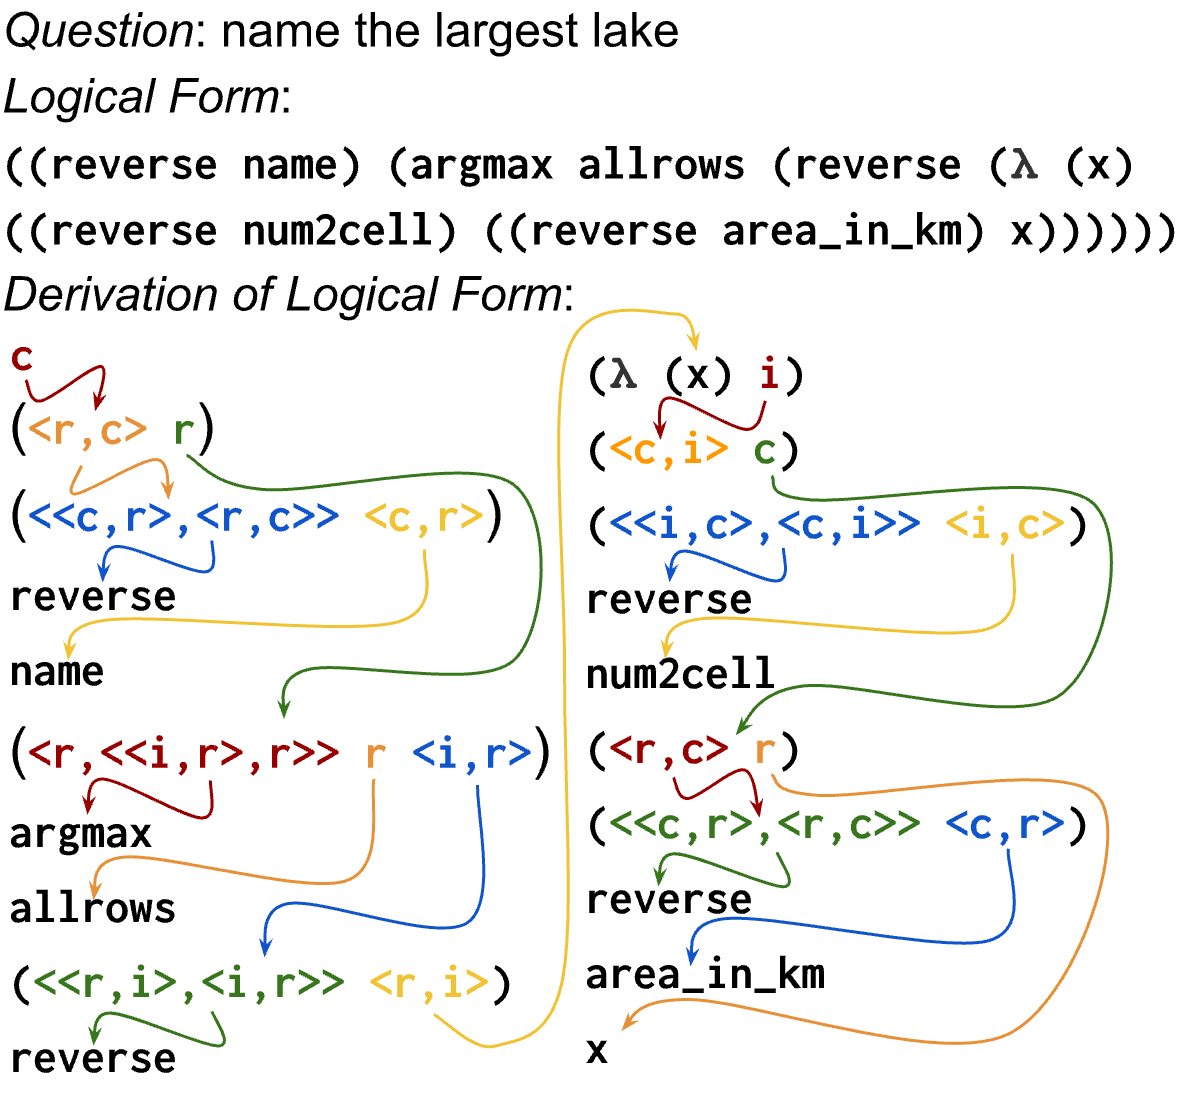
\includegraphics[width=3in]{figures/nnsp_example_derivation.png}
\caption{The derivation of a logical form using the  type-constrained grammar. 
The holes in the left column have 
empty scope, while holes in the right column have scope $\Gamma = \{(x : 
\type{r})\}$}
\label{fig:grammar_derivation}
\end{figure}

The first action of the parser is to predict a root type for the logical form, 
and then decoding proceeds according to the production rules above.
Each time step of decoding fills the leftmost hole in the logical form, and 
decoding terminates when no holes remain.
Figure \ref{fig:grammar_derivation} shows the sequence of decoder actions used 
to generate a logical form.

\paragraph{Network Architecture.} The decoder is an LSTM that outputs a 
distribution over grammar actions using an attention mechanism over the encoded 
question tokens. The decoder also uses a copy-like mechanism on the entity 
linking scores to generate entities.
Say that, during the $j$th time step, the current hole has type $\tau$. The 
decoder generates a score for each grammar action whose left-hand side is 
$\tau$ using the following equations:

\begin{align}
 (y_j, h_j) & = \text{LSTM}(h_{j-1}, \begin{bmatrix}g_{j-1} \\ 
o_{j-1}\end{bmatrix}) \label{eq:nnsp_decoder_lstm} \\
 a_j & = \text{softmax}(O W^a y_j) \label{eq:nnsp_decoder_lstm_output}\\
 o_j & = (a_j)^T O  \label{eq:nnsp_decoder_soft_att}\\
 s_j & = W^2_\tau \text{ ReLU}( W^1 \begin{bmatrix}y_j \\ o_j \end{bmatrix} + 
b^1) + b^2_\tau \label{eq:nnsp_score_rules}\\
 s_j(e_k) & = \sum_i s(e_k, i) a_{ji} \label{eq:nnsp_score_type}\\
 p_j & = \text{softmax}( \begin{bmatrix} s_j \\ s_j(e_1) \\ s_j(e_2) \\ ... 
\end{bmatrix} ) \label{eq:nnsp_score_action}
\end{align}

The input to the LSTM $g_{j-1}$ is a grammar action embedding for the action 
chosen in previous time step. $g_0$ is a learned parameter vector, and $h_0$ is 
the concatenated hidden states of the encoder LSTMs. The matrix $O$ contains 
the encoded token vectors $o_1, ..., ,o_n$ from the encoder. 
\Crefrange{eq:nnsp_decoder_lstm}{eq:nnsp_decoder_soft_att} above perform a 
softmax attention over $O$ using a learned parameter matrix $W^a$. 
Equation~\ref{eq:nnsp_score_rules} generates scores $s$ for the 
context-independent grammar rules applicable to type $\tau$ using a multilayer 
perceptron with weights $W^1$,$b^1$,$W^2_\tau$,$b^2_\tau$. 
Equation~\ref{eq:nnsp_score_type} generates a score for each entity $e$ with 
type $\tau$ by averaging the entity linking scores with the current attention 
$a_j$. Finally, the context-independent and -dependent scores are concatenated 
and softmaxed to produce a probability distribution $p_j$ over grammar actions 
in Equation~\ref{eq:nnsp_score_action}. If a context-independent action is 
chosen, $g_{j}$ is a learned parameter vector for that action. Otherwise $g_{j} 
= g^\tau$, which is a learned parameter representing the selection of an entity 
with type $\tau$.


\section{Experiments with \textsc{WikiTableQuestions}}
We now describe an application of our framework to \textsc{WikiTableQuestions}, 
a challenging dataset for question
answering against semi-structured Wikipedia tables 
\citep{pasupat2015compositional}. An example question from this dataset
is shown in Figure~\ref{fig:wikitables_example}.

\subsection{Context and Logical Form Representation}
\label{sec:preliminaries}

We follow \cite{pasupat2015compositional} in using the same table structure 
representation 
and $\lambda$-DCS language for expressing logical forms.
In this representation, tables are expressed as knowledge graphs over 6 types 
of 
entities: cells, cell parts, rows, columns, numbers and dates.
Each entity also has a name, which is typically a string value in the table.
Our parser uses both the entity names and the knowledge graph structure to 
construct embeddings for each entity. Specifically, the neighbors of a column 
are the cells it
contains, and the neighbors of a cell are the columns it belongs to.

The logical form language consists of a collection of named sets and entities, 
along with operators on them.
The named sets are used to select table cells, e.g., \pred{united\_states} is 
the set of cells that contain the text ``united states''.
The operators include functions from sets to sets, e.g., the \pred{next} 
operator maps a row to the next row.
Columns are treated as functions from cells to their rows, e.g., \pred{(country 
united\_states)} generates the rows whose \pred{country} column contains 
``united states''. 
Other operators include reversing relations (e.g., in order to map rows to 
cells 
in a certain column), relations that interpret cells as numbers and dates, and 
set and arithmetic operations. 
The language also includes aggregation and quantification operations such as 
\pred{count} and \pred{argmax}, along with $\lambda$ abstractions that can be 
used to join binary relations.

Our parser also assigns a type to every $\lambda$-DCS expression, which is used 
to enforce type constraints on generated logical forms.
The base types are cells \type{c}, parts \type{p}, rows \type{r}, numbers 
\type{i}, and dates \type{d}.
Columns such as \pred{country} have the functional type \func{c}{r}, 
representing functions from cells \type{c} to rows \type{r}.
Other operations have more complex functional types, e.g., \pred{reverse} has 
type
\func{\func{c}{r}}{\func{r}{c}}, which enables us to write \pred{(reverse 
country)}.\footnote{Technically, \pred{reverse} has the parametric polymorphic 
type \func{\func{\alpha}{\beta}}{\func{\beta}{\alpha}}, where \type{\alpha} and 
\type{\beta} are \emph{type variables} that can be any type. This type allows 
\pred{reverse} to reverse any function. However, this is a detail that can 
largely be ignored. We only use parametric polymorphism when typing logical 
forms to generate the type-constrained grammar; the grammar itself does not 
have 
type variables, but rather a fixed number of concrete instances -- such as 
\func{\func{c}{r}}{\func{r}{c}} -- of the above polymorphic type.}
The parser assigns every $\lambda$-DCS constant a type, then applies standard 
programming language type inference algorithms \citep{Pierce2002TypesAP} to 
automatically assign types to larger expressions.

\subsection{DPD Training}
\label{sec:nnsp_training}

Our parser is trained from question-answer pairs, treating logical forms as a 
latent variable. We use a new loglikelihood objective function for this process 
that first automatically enumerates a set of correct logical forms for each 
example, then trains on these logical forms. This objective simplifies the 
search problem during training and is well-suited to training our neural model.

The training data consists of a collection of $n$ question-answer-table 
triples, 
$\{(q^i, a^i, T^i)\}_{i=1}^n$. We first run dynamic programming on denotations 
\citep{pasupat2016inferring} on each table $T^i$ and answer $a^i$ to generate a 
set of 
logical forms $\ell \in \mathcal{L}^i$ that execute to the correct answer.

\paragraph{Dynamic programming on denotations.} DPD is an automatic procedure for enumerating 
logical forms that execute to produce a particular value; it leverages the 
observation that there are fewer denotations than logical forms to enumerate 
this set relatively efficiently. It is a kind of chart parsing algorithm where
partial parses are grouped together in cells by their output category, size, and
the denotation. This is an improvement over the previous work by \cite{pasupat2015compositional},
where the logical forms were grouped based on only the output category and size.
Given this chart, DPD performs two forward passes, In the first pass, the algorithm
finds all the cells that lead to the correct denotation. In the second pass, all the
rule combinations which lead to the cell corresponding to the correct denotation
are listed, and logical forms are generated from those cells, using only the rule combinations
that are known to lead to the final cells.

Given the logical forms generated from DPD, we train the model 
with the following objective: 

\begin{align}
    \mathcal{O}(\theta) & = \sum_{i=1}^n \log \sum_{\ell \in \mathcal{L}^i} 
P(\ell | q^i, T^i; \theta )
\end{align}

We optimize this objective function using stochastic gradient descent.
If $|\mathcal{L}^i|$ is small, e.g., 5-10, the gradient of the $i$th example 
can 
be computed exactly by simply replicating the parser's network architecture 
$|\mathcal{L}^i|$ times, once per logical form.
(Note that this takes advantage of the property that each logical form has a 
unique derivation in the decoder's grammar.)
However, $|\mathcal{L}^i|$ often contains many thousands of logical forms, 
which 
makes the above computation infeasible. We address this problem by truncating 
$\mathcal{L}^i$ to the $m=100$ shortest logical forms, then using a beam search 
with a beam of $k=5$ to approximate the sum.

We briefly contrast this objective function with two other commonly-used 
approaches. The first approach is commonly used in prior semantic parsing work 
with loglinear models \citep{Liang2011LearningDC,pasupat2015compositional} and 
uses a similar 
loglikelihood objective. The gradient computation for this objective requires 
running a wide beam search, generating, e.g., 300 logical forms, executing each 
one to identify which are correct, then backpropagating through a term for 
each. 
This process would be very expensive with a neural model due to the cost of 
each 
backpropagation pass. Another approach is to train the network with REINFORCE 
\citep{williams1992simple}, which essentially samples a logical form instead of 
using 
beam search. This approach is known to be difficult to apply when the space of 
latent variables is large and the reward signal sparse, as it is in semantic 
parsing. Our objective improves on these by precomputing correct logical forms 
in order 
to avoid searching for them during the gradient computation.

\subsection{Experimental Setup}
We used the standard train/test splits of \textsc{WikiTableQuestions}.
The training set consists of 14,152 examples and the test set consists of 4,344 
examples.
The training set comes divided into 5 cross-validation folds for development 
using an 80/20 split.
All data sets are constructed so that the development and test tables are not 
present in the training set.
We report question answering accuracy measured using the official evaluation 
script, which performs some simple normalization of numbers, dates, and strings 
before comparing predictions and answers.
When generating answers from a model's predictions, we skip logical forms that 
do not execute (which may occur for some baseline models) or answer with the 
empty string (which is never correct).
All reported accuracy numbers are an average of 5 parsers, each trained on one 
training fold, using the respective development set to perform early stopping.

We trained our parser with 20 epochs of stochastic gradient descent. We used 
$200$-dimensional word embeddings for the question and entity tokens, mapping 
all tokens that occurred $<3$ times in the training questions to \texttt{UNK}. 
(We tried using a larger vocabulary that included frequent tokens in tables, 
but this caused the parser to seriously overfit the training examples.) The 
hidden and output dimensions of the forward/backward encoder LSTMs were set to 
$100$, such that the concatenated representations were also $200$-dimensional. 
The decoder LSTM uses $100$-dimensional action embeddings and has a 
$200$-dimensional hidden state and output. The action selection MLP has a 
hidden layer dimension of $100$. We used a dropout probability of $0.5$ on the 
output of both the encoder and decoder LSTMs, as well as on the hidden layer of 
the action selection MLP. At test time, we decode with a beam size of 10.

\subsection{Results}
Table \ref{tab:nnsp_wikitables_results} compares the accuracy of our semantic parser 
to prior work on \textsc{WikiTableQuestions}.
We distinguish between single models and ensembles, as we expect ensembling to 
improve accuracy, but not all prior work has used it.
Prior work on this data set includes a loglinear semantic parser 
\citep{pasupat2015compositional}, that same parser with a neural, paraphrase-based reranker 
\citep{haug2017neural}, and a neural programmer that answers questions by predicting a 
sequence of table operations \citep{Neelakantan2016LearningAN}.  
We find that our parser outperforms the best prior result on this data set by 
4.6\%, despite that prior result using a 15-model ensemble.
An ensemble of 5 parsers, one per training fold, improves accuracy by an 
additional 2.6\% for a total improvement of 7.2\%.
\begin{table}
    \centering
    \begin{tabular}{|l|c|c|c|}
	\hline
        \textbf{Model} & \textbf{Ensemble Size} & \textbf{Dev.} & \textbf{Test} \\
        \hline 
        \cite{Neelakantan2016LearningAN} & 1 & 34.1 & 34.2 \\
        \cite{haug2017neural} & 1 & - & 34.8 \\
        \cite{pasupat2015compositional} & 1 & 37.0 & 37.1 \\
        \cite{Neelakantan2016LearningAN} & 15 & 37.5 & 37.7 \\
        \cite{haug2017neural} & 15 & - & 38.7 \\
        \hline
        Our Parser & 1 & 42.7 & 43.3 \\
        Our Parser & 5 & - & \textbf{45.9} \\
        \hline
    \end{tabular}
    \caption{Development and test set accuracy of our semantic parser compared to prior work on \textsc{WikiTableQuestions}}
    \label{tab:nnsp_wikitables_results}
\end{table}

\section{Proposed Work}
The initial results with our framework on a difficult dataset show that this is a promising direction for building weakly
supervised semantic parsers for reasoning over structured or semi-structured domains. We now list out the directions for
proposed work in this chapter.

\subsection{Handling more operations and improved entity linking}
While the results in Table~\ref{tab:nnsp_wikitables_results} show that the proposed framework outperforms previous systems,
the absolute accuracy of the system shows that there is still room for improvement. Following are some improvements that can be made to improve
performance on this dataset.

Our entity embedding and linking module
described in Section~\ref{sec:nnsp_encoder} is fairly simple, and does not account for paraphrases of predicates seen in questions
(like ``go to'' referring to ``attended'' in the context of attending an academic institution), or abbreviations used for entities
(like ``DNQ'' for ``did not qualify'') etc.

Moreover, on close examination of the errors made by the parser on a sample of 100 questions from the \textsc{WikiTableQuestions} dataset,
we found that a major class of errors (26.5\%) is on questions that place explicit set membership constraints on outputs. Following are
two examples of such questions:
\begin{itemize}
 \item In 2008, in track and field events who broke more world records, Usain Bolt or Haile Gebrselassie?
 \item What vehicle maker other than Dodge has the most vehicles in the roster?
\end{itemize}
Both the questions above specify sets of entities and the parser should operate on those sets instead of all those in the context. One way of achieving this
is by introducing set membership operations in the grammar.

\subsection{Extending to datasets with weaker supervision}
The method described in this chapter relies strongly on DPD. An assumption we make here is that supervision in the 
form of the right answer is sufficient to enumerate the set of correct logical forms. However, this may not be true in all cases. For example, the Cornell
Natural Language Visual Reasoning (NLVR)\footnote{\url{http://lic.nlp.cornell.edu/nlvr/}} \citep{suhr2017corpus} dataset is a set of natural language utterances grounded in (synthetically generated) images,
and the task is to answer whether the utterance is true or false. Figure~\ref{fig:nnsp_nlvr_example} shows an example. Since the supervision is available is
in the form of a binary label, it may be significantly more challenging to run DPD on this dataset. We expect the output thus generated will contain a very large number
of spurious logical forms (those that are incorrect, but execute to the correct denotation), and hence will affect our training process adversely.
\begin{figure}
  \begin{center}
  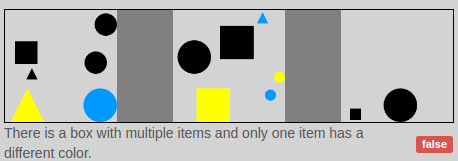
\includegraphics[width=4in]{figures/nlvr_example.png}
  \caption{Example from NLVR Dataset}
  \label{fig:nnsp_nlvr_example}
  \end{center}
\end{figure}

To address this problem, we will investigate constraining DPD to generate logical forms grounded in the input utterance. As described in
Section~\ref{sec:nnsp_training}, DPD consists of two passes, and the second pass involves using all rule combinations that lead to the
cells with correct denotations. One possibility to constrain this process is to score the rule combinations conditioned on the input
utterance.
